\chapter{Установка и настройка iRedMail}
\label{ch:practice}

\section{Загрузка iRedMail}

На ВМ \texttt{mail} скачиваем архив iRedMail версии~1.6.2
с официального репозитория GitHub:

\begin{lstlisting}
apt-get update
wget https://github.com/iredmail/iRedMail/archive/refs/tags/1.6.2.tar.gz
tar xvf 1.6.2.tar.gz
\end{lstlisting}

\section{Предварительная загрузка пакетов}

Перед запуском интерактивного установщика загружаем необходимые
пакеты в автоматическом режиме:

\begin{lstlisting}
cd iRedMail-1.6.2/
cd pkgs/
chmod +x get_all.sh
./get_all.sh
\end{lstlisting}

\section{Запуск установщика iRedMail}

Возвращаемся в корень распакованного дистрибутива и запускаем
интерактивный установщик:

\begin{lstlisting}
cd ..
chmod +x iRedMail.sh
./iRedMail.sh
\end{lstlisting}

Установщик задаёт ряд вопросов через текстовый интерфейс.
Ниже приведены рекомендуемые ответы для данного варианта.

\subsection{Выбор веб-сервера}

Установщик предлагает выбрать веб-сервер: \textbf{Nginx} или Apache.
Выбираем \textbf{Nginx}.

\subsection{Выбор бэкенда для пользователей}

Установщик предлагает тип хранилища учётных записей.
Выбираем \textbf{OpenLDAP};
в поле \textit{LDAP suffix} вводим:

\begin{lstlisting}
\cfgLdapSuffix
\end{lstlisting}

\subsection{Завершение установки}

После прохождения всех экранов установщик производит автоматическую
установку и настройку всех компонентов. По завершении появляется
сообщение об успешной инсталляции.

Установщик сообщает учётные данные администратора:\\
\texttt{postmaster@\cfgDomain}.

\section{Проверка статуса сервисов}

После завершения установки перезагружаем машину и проверяем
состояние ключевых сервисов:

\begin{lstlisting}
reboot
\end{lstlisting}

\begin{lstlisting}
systemctl status postfix
systemctl status dovecot
systemctl status nginx
\end{lstlisting}

Все три сервиса должны находиться в состоянии \texttt{active (running)}.

% — Скриншот: systemctl status postfix (active running) —
\begin{figure}[h]
  \centering
  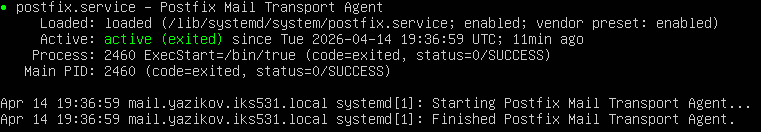
\includegraphics[width=0.85\textwidth]{img/06_postfix_status}
  \caption{Статус \texttt{postfix} — active (running)}
  \label{fig:postfix_status}
\end{figure}

% — Скриншот: systemctl status dovecot (active running) —
\begin{figure}[h]
  \centering
  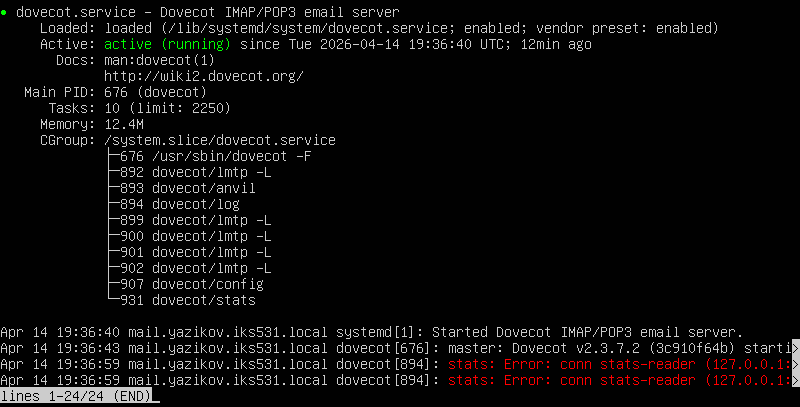
\includegraphics[width=0.85\textwidth]{img/07_dovecot_status}
  \caption{Статус \texttt{dovecot} — active (running)}
  \label{fig:dovecot_status}
\end{figure}

\section{Проверка веб-интерфейса}

\subsection{Панель администратора iRedAdmin}

С браузера Desktop переходим по адресу:

\begin{lstlisting}
https://mail.\cfgDomain/iredadmin
\end{lstlisting}

Входим с учётными данными:\\
\textit{Логин:}\\ \texttt{postmaster@\cfgDomain},\\
\textit{Пароль:} указанный при установке.

% — Скриншот: браузер Desktop, страница авторизации iRedAdmin —
\begin{figure}[h]
  \centering
  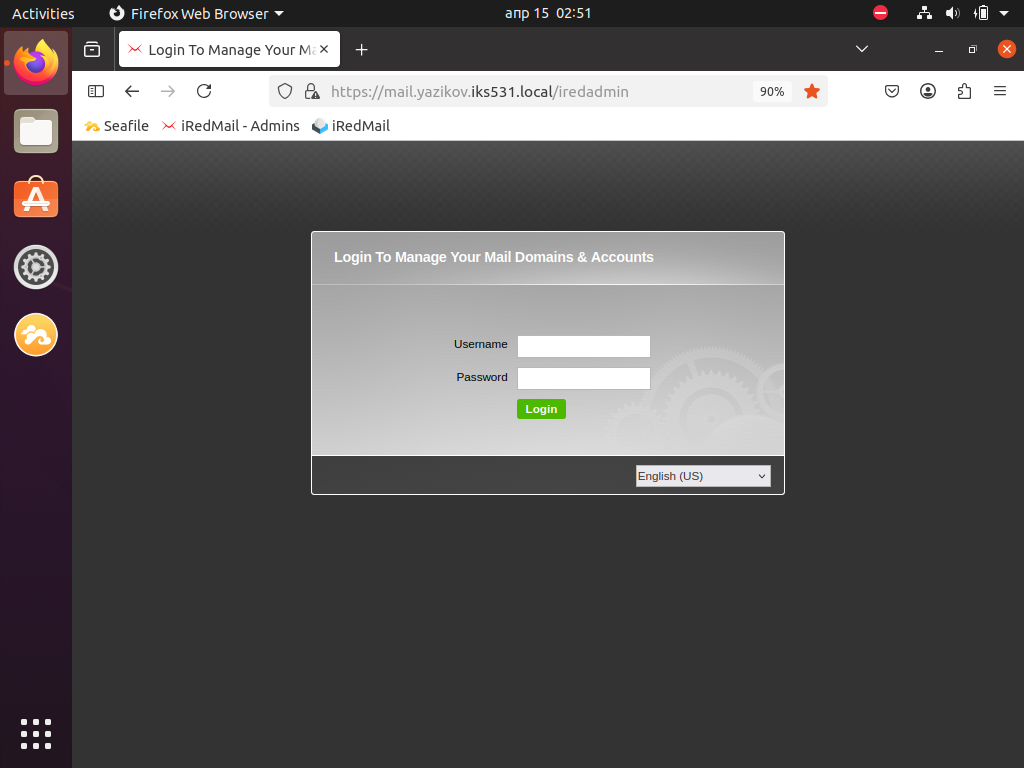
\includegraphics[width=0.85\textwidth]{img/08_iredadmin_login}
  \caption{Страница авторизации панели \texttt{iRedAdmin}}
  \label{fig:iredadmin_login}
\end{figure}

% — Скриншот: дашборд iRedAdmin после входа —
\begin{figure}[h]
  \centering
  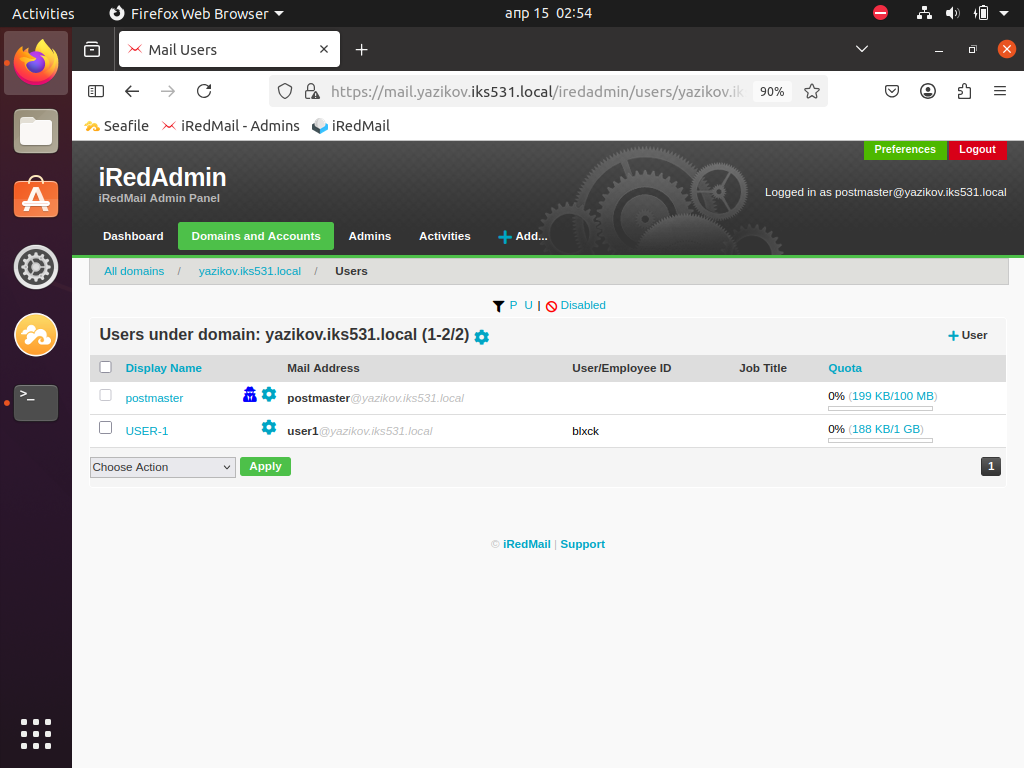
\includegraphics[width=0.85\textwidth]{img/09_iredadmin_dashboard}
  \caption{Главная панель \texttt{iRedAdmin} — домен и пользователи}
  \label{fig:iredadmin_dash}
\end{figure}

\subsection{Веб-клиент Roundcube}

Для входа в почтовый клиент переходим по адресу:

\begin{lstlisting}
https://mail.\cfgDomain/mail
\end{lstlisting}

% — Скриншот: страница авторизации Roundcube —
\begin{figure}[h]
  \centering
  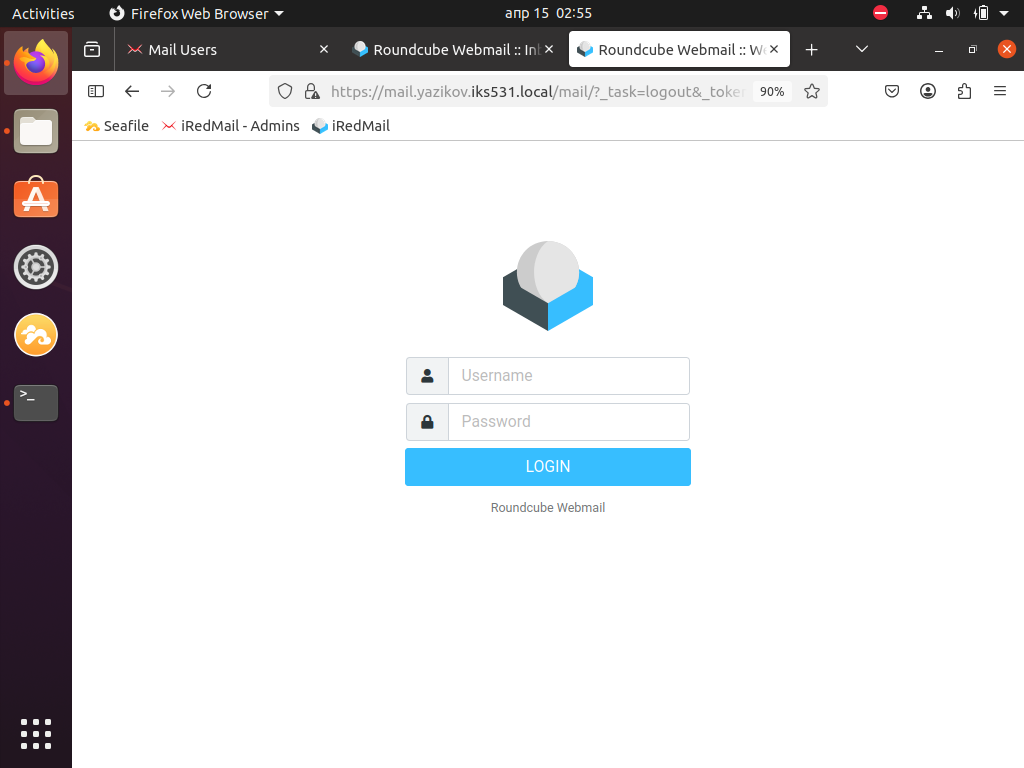
\includegraphics[width=0.85\textwidth]{img/10_roundcube_login}
  \caption{Страница авторизации \texttt{Roundcube Webmail}}
  \label{fig:roundcube_login}
\end{figure}

\endinput
